\documentclass[11pt]{article}

\input{../../preamble.tex}
% --- Page geometry tuned to match the PDF look ---
\usepackage[margin=1.2in]{geometry}
\usepackage{amsmath,amssymb,amsfonts}
\usepackage{enumitem}
\usepackage{mathtools}
\usepackage{graphicx}

\setlength{\parindent}{0pt}
\setlength{\parskip}{6pt}

\newcommand{\ellinfty}{\ell^{\infty}}
\newcommand{\ellone}{\ell^{1}}
\newcommand{\ellzero}{\ell_{0}}
\newcommand{\ellc}{\ell_{c}}
\newcommand{\norm}[1]{\left\lVert #1 \right\rVert}
\newcommand{\restr}[2]{#1\!\upharpoonright_{#2}}

\usepackage{cancel}


\begin{document}

\begin{center}
    {\LARGE Math 421/510: Homework 5}
\end{center}

\vspace{1.5em}

\begin{enumerate}[leftmargin=2em, label=\arabic*.]
    \item Given $\phi:\mathbb{R}\to\mathbb{R}$ we define the function $f_{r,\delta}:\mathbb{R}^2\to\mathbb{R}$ by
    \[
    f_{r,\delta}(x,y)=\frac{1}{r}\phi\!\left(\frac{x}{r}\right)\frac{1}{\delta}\phi\!\left(\frac{y}{\delta}\right).
    \]

    \begin{enumerate}[label=(\alph*), leftmargin=2em]
        \item Let $\phi:\mathbb{R}\to\mathbb{R}$ be a continuous function such that
        \[
        \operatorname{supp}\phi \subseteq [-2,2], \qquad \phi(x)=1 \text{ for } x\in[-1,1].
        \]
        Let $r,\delta>0$, assume $r$ is large and $\delta$ is small, and Note that $f_{r,\delta}$ is essentially supported/concentrated in a horizontal rectangle of size $\sim r\times \delta$. Compute $\widehat{f_{r,\delta}}$ and determine where it is concentrated in frequency space.

        \item Choose an explicit function of $\phi$ satisfying the assumptions above (Hint: if you choose a trapezoidal bump function, it can be written as a convolution of two characteristic functions on an interval) and compute $\widehat{\phi}$ explicitly. Use this example to illustrate the concentration properties found in part (a) and check Plancherel's identity for $f_{r,\delta}$.

        \item Repeat (a) and (b) for the case $\phi(x)=e^{-x^2}$. Compute the Fourier transform explicitly and verify Plancherel in this case.

        \item Do the conclusions become stronger if $\phi$ is smoother? Justify your answer.
    \end{enumerate}

    \textbf{Solution.}
    \begin{enumerate}
        \item We compute $\widehat{f_{r, \delta}}$.
            We justify the use of Fubini Tonelli since $f_{r, \delta}e^{-2\pi i \xi \cdot x}$ is compactly supported and bounded so it is in $L^{1}$.
            \begin{align*}
                \widehat{f_{r, \delta}}(\xi_{x}, \xi_y) &=  \int_{\R^{2}} f_{r, \delta}(x, y) e^{-2\pi i x \xi_{x}}  e^{-2\pi i y \xi_{y}} \\
                &=  \int_{\R^2} \frac{1}{r} \phi(x / r) \frac{1}{\delta} \phi(y / \delta) e^{-2\pi i x \xi_{x}}  e^{-2\pi i y \xi_{y}} \\
                &= \int_{\R} \frac{1}{r} \phi(x / r) e^{-2\pi i x \xi_{x}} dx\int_{\R} \frac{1}{\delta} \phi(y / \delta) e^{-2\pi i y \xi_{y}} dy \text{ by Fubini-Tonelli}\\
                &=  \int_{\R} \phi(u) e^{-2 \pi i \xi_{x} r u } du \int_{\R} \phi(v) e^{- 2 \pi i \delta v \xi_y} dv \\
                &= \hat{\phi}(r \xi_x) \hat{\phi}(\delta \xi_y) 
            .\end{align*}
            Since $\phi$ is in $L^{1}$, we have that $\hat{\phi} \in C_{0}$.
            Therefore, for any $\epsilon > 0$ there exists some interval $[-M, M]$ such that $\int_{\R \setminus [-M, M]} |\hat{\phi}| < \epsilon$.

            But then, $\hat{\phi}(r \xi_x)$ is concentrated in the interval $[-M / r, M / r]$, and $\hat{\phi}(\delta \xi_y)$ is concentrated in $[-\delta M / \delta, \delta M / \delta]$.
            If $r$ is large and $\delta$ is small, this means that the rectangle $[(-rM, -\delta M), (rM, \delta M)]$ in which $\widehat{f_{r, \delta}}$ is concentrated has a small dimension in the $\xi_x$ frequency axis and a short dimension in the $\xi_y$ frequency axis.
            Thus, it is concentrated close to the $\xi_x$ axis in frequency space.
        \item We consider $g = \chi_{[-1, 0]}$, and $h = \chi_{[-2, 1]}$.
            We compute $g * h$ to show that it has the desired properties.
            \begin{align*}
                g * h(x) &= \int_{\R} g(x - y) h(y) dy\\
                      &= \int_{-2}^{1} \chi_{[-1, 0]}(x - y)dy \\
                      &= \int_{-2}^{1} \chi_{[-1 - x, -x]}(-y)dy
            .\end{align*}
            If $|x| > 2$, then $-1 - x > 1$ or $-x < -2$, which will mean $\chi_{[-1 - x, -x]}$  is disjoint with the domain of integration, so we have $g * h (x ) = 0$.
            Now, suppose that $-2 \le x \le  -1$. Then,
            \[
            g * h(x) = \int_{-2}^{1} \chi_{[-1 - x, -x]}(-y)dy = \int_{-1 - x}^{1}dy = 1 + 1 - x \implies 0 \leq  g * h (x) \leq 1
            .\] 
            Suppose $-1 \leq x \leq 1$. Then,
            \[
            g * h(x) = \int_{-2}^{1} \chi_{[-1 - x, -x]}(-y)dy = \int_{-1 - x}^{-x}dy = -x + 1 + x = 1 \implies  g * h (x) = 1
            .\] 
            Finally, suppose $1 \leq x \leq 2$. Then,
            \[
            g * h(x) = \int_{-2}^{1} \chi_{[-1 - x, -x]}(-y)dy = \int_{-2}^{-x}dy = -x + 2 \implies 0 \leq  g * h (x) \leq 1
            .\] 
            Since the convolution of $L^{1}$ functions is continuous, we have that $g^{*}$ is continuous, $g*h(x) = 1$ for $x \in [-1, 1]$ (as desired), and $\mathrm{supp} \phi \subseteq [-2, 2]$.

            Now, if $\phi = g * h$, then $\hat{\phi} = \hat{g} \hat{h}$.
            We have that:
            \begin{align*}
                \hat{g} &= \frac{1}{-2\pi i \xi} (1 - e^{2\pi i \xi}) = \frac{1}{\pi \xi} e^{\pi i \xi} \sin(\pi \xi)\\
                \hat{h} &= \frac{1}{-2 \pi i \xi} (e^{-2 \pi i \xi} - e^{4 \pi i \xi}) = \frac{1}{\pi \xi} e^{-\pi i \xi} \sin(3 \pi \xi)
            .\end{align*}
            So, $\hat{g}\hat{h} = \frac{1}{\pi^2 \xi^2}\sin(\pi \xi) \sin(3 \pi \xi)$

            Then, we have that
            \[
                \widehat{f_{r,\delta}}(\xi_x, \xi_y) =  \frac{1}{\pi^{4} r^2 \delta^2 \xi_x^{2} \xi_y^2} \sin(r 3 \pi \xi_x) \sin(r \pi \xi_x) \sin(\delta \pi \xi_y) \sin(\delta 3 \pi \xi_y)
            .\] 
            Close to the origin, we have that $\sin(\xi) \approx \xi$, so then $\frac{1}{\pi^2 \xi^2} \sin(\pi\xi) (3\pi \xi) \approx 3$.
            When $\xi > 1$ however, the function quickly drops off to zero.
            Here is the function in Desmos:
            \begin{figure}[h]
                \centering
                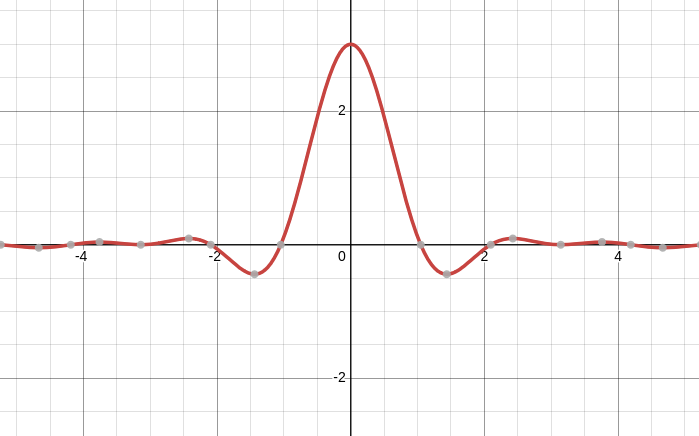
\includegraphics[width=0.7\textwidth]{bump.png}
                \caption{$\frac{1}{\pi^2 x^2}\sin(\pi x)\sin(3\pi x)$}
                \label{fig:bump}
            \end{figure}

            How "wide" this bump is, and how close it is to the $\xi_x$ and $\xi_y$ axes, is then determined by these scaling factors $\delta, r$ in the respective dimensions.
            Thus, the bump will be situated in the rectangle $[(-1/r, -1 / \delta), (1 / r, 1 / \delta)]$.

            Finally, we check Plancherel's identity.
            Since $f$ and $g$ are linear functions, their convolution is a trapezoid.
            In this case, we can easily see that the area of the trapezoid is $\int_{-2}^{2}\phi(x) = 1 / 2 + 2 + 1 / 2 = 4$.
            The area under the squared trapezoid, is then $\int_{-2}^{2} |\phi(x)|^2 = \frac{1}{3} + 2 + \frac{1}{3} = 8 / 3$.
            Then,
            \begin{align*}
                \int_{\R^2} |f_{r, \delta}|^2 &= \int_{\R} \frac{1}{r^2} |\phi(x / r)|^2 dx \int_{\R} \frac{1}{\delta^2} |\phi(y / \delta)|^2 dy\\
                &= \frac{1}{r \delta} \int_{\R} |\phi(x)|^2 \int_{\R} |\phi(y)|^2dy = \frac{64}{9 r \delta}
            .\end{align*}
            I'm afraid I will have to take the L on the integral in the frequency domain\ldots I'm not sure how to tackle it.

        \item By Theorem 5.5 in class, we have that $\mathcal{F}(\phi) = \mathcal{F}(e^{-x^2}) = \frac{1}{\sqrt{\pi}} e^{- \pi^2 \xi^2}$, since here $a = 1 / \pi$.
            Thus,
            \[
                \widehat{f_{r,\delta}}(\xi_x, \xi_y) = \frac{1}{\pi}  e^{-\pi^2 ((r\xi_x)^2 + (\delta \xi_y)^2)}
            .\] 

            We use Fubini freely.
            Now, we verify Plancherel.
            \begin{align*}
                \int_{\R^2} |f_{r, \delta}|^2 = \frac{1}{r^2 \delta^2} \int_{\R} e^{-2x^2 / r^2} dx \int_{\R} e^{-2y^2 / \delta^2} dy = \frac{1}{r^2 \delta^2}\left( \sqrt{\frac{r^2}{2 \pi} }\right) \left( \sqrt{\frac{\delta^2}{2 \pi}}\right) = \frac{1}{r \delta} \frac{1}{2 \pi}
            .\end{align*}

            Next, we compute:
            \begin{align*}
                \int_{\R^2} |\widehat{f_{r, \delta}}|^2 = \int_{\R} \frac{1}{\pi} e^{-2\pi^2r^2\xi_x^2} d\xi_x \int_{\R} \frac{1}{\pi} e^{-2\pi^2\delta^2\xi_y^2} d\xi_y = \frac{1}{\pi} \left( \sqrt{\frac{\pi}{2 r^2}}\right) \left( \sqrt{\frac{\pi}{2 \delta^2}}\right) = \frac{1}{r \delta} \frac{1}{2\pi}
            .\end{align*}
            Thus, we have verified Plancherel's identity.


        \item If $\phi$ becomes smoother, then by theorem 5.10 5) $\hat{\phi}$ decays at least as quickly as the power of the highest degree continuous derivative.
            We can say more precisely how the frequency spectrum will decay. We don't just know that it eventually will (which is what the Riemann-Lebesuge lemma means, in having $\mathcal{F}(L^{1}) \subset C_0$).

    \end{enumerate}


    \item On $\mathbb{R}$, let
    \[
    f(x)=
    \begin{cases}
        2x+1 & -\frac{1}{2}\leq x\leq 0,\\
        1-2x & 0\leq x\leq \frac{1}{2},\\
        0 & |x|>\frac{1}{2}.
    \end{cases}
    \]

    \begin{enumerate}[label=(\alph*), leftmargin=2em]
        \item Show that
        \[
        \widehat{f}(\xi)=\frac{1-\cos(\pi \xi)}{\pi^2 \xi^2}.
        \]

        \item Briefly explain why this computation is consistent with the principle quantified by the relations
        $ \widehat{g^{(n)}}(\xi)=(2\pi i\xi)^n\widehat{g}(\xi)$
        and
        $(-2\pi i x)^n g(x) = (\widehat{g})^{(n)}(\xi)$
    that spatial decay of a function is reflected in the smoothness of its Fourier transform (and vice versa).

        \item Use your computation from part (a) to show:
        \begin{enumerate}[label=\roman*., leftmargin=2em]
            \item $\displaystyle \sum_{n=0}^{\infty}\frac{1}{(2n+1)^2}=\frac{\pi^2}{8};$
            \item $\displaystyle \sum_{n=0}^{\infty}\frac{1}{(2n+1)^4}=\frac{\pi^4}{96}.$
        \end{enumerate}
    \end{enumerate}



    \begin{enumerate}
        \item First, note that $f(x)= \chi_{[-1 / 2, 1 / 2]} + 2x\chi_{[-1 / 2, 0]} - 2x \chi_{[0, 1 / 2]}$

            We compute:
            \begin{align*}
                \hat{f}(\xi) &= \int_{\R} f(x) e^{-2  \pi i x \xi } dx \\
                &= \int_{-1 / 2}^{1 / 2} e^{-2 \pi i x \xi}dx + \int_{-1 / 2}^{0} 2x e^{-2 \pi i x \xi} dx - \int_{0}^{1 / 2} 2x e^{-2\pi i x \xi}
            .\end{align*}
            The first integral is just $\frac{1}{-2\pi i \xi}e^{-2 \pi i x \xi} \bigg|_{- 1 / 2}^{1 / 2} = \frac{1}{-2 \pi i \xi} (e^{- \pi i \xi} - e^{\pi i \xi}) = \frac{1}{i \pi \xi} \sin(\pi \xi)$.
            The next two integrals, by integration by parts, is
            \begin{align*}
                \int_{a}^{b} 2x e^{-2\pi i x \xi} &= \frac{2x}{-2\pi i \xi} e^{- 2 \pi i x \xi} \bigg|_{a}^{b} - \int_{a}^{b} \frac{1}{- \pi i \xi} e^{- 2\pi i x \xi} dx \\ 
                &= \frac{1}{-\pi i \xi}(b e^{-2 \pi i b \xi} - a e^{-2 \pi i a \xi}) - \frac{1}{-2\pi^2 \xi^2} e^{-2\pi i x \xi} \bigg|_{a}^{b}
            .\end{align*}
            Plugging this in with the respective bounds $-1/2, 0$ and $0, 1 / 2$, we get
            \begin{align*}
                \hat{f}(\xi) &= \frac{1}{\pi i \xi} \sin(\pi \xi) + \left(\frac{1}{-2\pi i \xi} e^{\pi i \xi} + \frac{1}{2 \pi^2 \xi^2}(1 - e^{\pi i \xi})\right) - \left( -\frac{1}{2\pi i \xi}e^{-\pi i \xi} + \frac{1}{2\pi^2 \xi^2} (e^{-\pi i \xi} - 1) \right)\\
                &= \frac{1}{\pi i \xi}\sin(\pi \xi) - \frac{1}{\pi i \xi}\sin(\pi \xi) + \frac{1}{\pi^2 \xi^2}(1 - \frac{1}{2} e^{\pi i \xi} - \frac{1}{2} e^{-\pi i \xi}) \\
                &=  \frac{1}{\pi^2 \xi^2} (1 - \cos(\pi \xi))
            ,\end{align*}
            as desired.
            Also, we note that since the fourier transform is uniformly continuous when $f$ is in $L^{1}$ (as is the case here), we compute $\hat{f}(0)$ by a double application of l'Hopital's rule:
            \[
                \hat{f}(0) = \lim_{\xi \to 0} \hat{f}(\xi) = \frac{\lim_{\xi \to 0}( 1 - \cos(\pi \xi))}{\lim_{\xi \to 0}\pi^2 \xi^2}  = \frac{\lim_{\xi \to 0} \pi \sin(\pi \xi)}{\lim_{\xi \to 0}2 \pi^2 \xi} = \frac{\lim_{\xi \to 0} \pi^2 \cos(\pi \xi)}{\lim_{\xi \to 0} 2\pi^2} = \frac{1}{2}
            .\] 
        \item Since $f$ is not particularly smooth (it doesn't have a continuous derviative\ldots it is continuous, but the only gaurantee that gives us is that the fourier transform is in $C_{0}$), we can't say much about it.
            However, $f$ has immediate spacial decay. Indeed, it is in $C_c$, when we see that $\mathrm{supp}{f} = [-1, 1]$.
            Therefore, it checks out tha $\hat{f}$ is infinitely differentiable (in $C^{\infty}$).
        \item 
            \begin{enumerate}
                \item 

                    First, we recognize that $f$ is continuous at $0$, since $2(0) + 1 = 1 - 2(0) = 1$, and since $|\hat{f}(k)| \leq \frac{2}{\pi^2 k^2}$ for each $k > 0$, we have that
                    \[
                        \sum_{k \in \Z} | \hat{f}(k)| \leq \frac{1}{2} +2 \cdot \frac{2}{\pi^2 \xi^2}  \sum_{n = 1}^{\infty} \frac{1}{k^2} < \infty
                    .\] 
                    Therefore, we can apply the Poisson summation formula, since it's conditions are satisfied.
                    But since $f(x) = 0$ for $|x| > 1 / 2$, we have $\sum_{m \in \Z} f(m) = f(0)$.
                    Also, for $k \in \Z$, we have that $\frac{1 - \cos(\pi k)}{\pi^2k^2} = 0$ when $k$ is non-zero even and $\frac{2}{\pi^2 k^2}$ when $k$ is odd.
                    Thus,
                    \begin{align*}
                        \sum_{k \in \Z} \hat{f}(k) &= \hat{f}(0) + 2\cdot \sum_{k = 1}^{\infty} \hat{f}(k)  \text{ since $\hat{f}$ is an even function}\\
                                                   &= \frac{1}{2} + 2\cdot \sum_{n = 0}^{\infty} \hat{f}(2n + 1) \text{ since $\hat{f}(k) = 0$ when $k$ even } \\
                                                   &= \frac{1}{2} + 2 \frac{1}{\pi^2} \sum_{n = 0}^{\infty} \frac{2}{(2n + 1)^2}
                    .\end{align*}
                    Applying the Poisson integral formula,
                    \begin{align*}
                        \sum_{m \in \Z} f(m) &= \sum_{k \in \Z} \hat{f}(k)\\
                        1 &= \frac{1}{2} + 2 \frac{1}{\pi^2} \sum_{n = 0}^{\infty} \frac{2}{(2n + 1)^2}\\
                        \frac{1}{2} &= \frac{4}{\pi^2} \sum_{n= 0}^{\infty} \frac{1}{(2n + 1)^2}\\
                        \implies \frac{\pi^2}{8} &= \sum_{n = 0}^{\infty} \frac{1}{(2n + 1)^2}
                    ,\end{align*}
                    as desired.
                \item 
                    First, we see that
                    \begin{align*}
                        \|Pf\|^2_{L^2(\mathbb{T})} = \int_{\R} |f|^2 &= \int_{-1 / 2}^{0} (2x + 1)^2 + \int_{0}^{1 / 2} (1 - 2x)^2\\
                        &= \frac{1}{2}\int_{0}^{1}u^2 du - \frac{1}{2} \int_{1}^{0}u^2 du \\
                        &= \frac{1}{6} + \frac{1}{6} = \frac{1}{3}
                    .\end{align*}
                    By Theorem 5.33, $\widehat{Pf}(k) = \hat{f}(k)$, and by the Parseval identity, we have $\sum_{k \in \Z} |\hat{f}(k)|^2 = \|Pf\|^2_{L^2(\mathbb{T})}$.
                    Arguing similarly about the eveness of $\hat{f}$ and how it is zero on the non-zero even integers, we compute this sum:
                    \begin{align*}
                        \sum_{k \in \Z} |\hat{f}(k)|^2 &= \frac{1}{2^2} + 2 \cdot \sum_{n = 0}^{\infty} |\hat{f}(2n + 1)|^2\\
                        &= \frac{1}{2^2} + 2\cdot \sum_{n= 0}^{\infty} \frac{4}{\pi^{4}(2n + 1)^{4}}  \\
                        &= \frac{1}{4} + \frac{8}{\pi^{4}} \sum_{n = 0}^{\infty} \frac{1}{(2n + 1)^{4}}
                    .\end{align*}
                    With Parseval, we get
                    \begin{align*}
                        \frac{1}{3} &= \frac{1}{4} + \frac{8}{\pi^4} \sum_{n= 0}^{\infty} \frac{1}{(2n + 1)^{4}}\\
                \frac{1}{12} &= \frac{8}{\pi^4} \sum_{n =0}^{\infty} \frac{1}{(2n + 1)^{4}}\\
                \frac{\pi^{4}}{96} &= \sum_{n =0}^{\infty} \frac{1}{(2n + 1)^{4}}
                    ,\end{align*}
                    as desired.
            \end{enumerate}
    \end{enumerate}

\end{enumerate}

\end{document}
